\section{The Hera mission}
\label{intro}
Cruising some 250 million kilometers around the Sun is an object first identified in 1996 as 1196G, by a Spacewatch survey at the  University of Arizona. It was later named Didymos (Greek word for twin), after a smaller companion, Didymoon, was discovered orbiting it. Didymos is now classified  as a potentially hazardous, near-Earth system. 
Hera, named after the greek goddess of marriage, will be humanity's first probe to rendezvous with a binary asteroid system. 

Hera is part of an international collaboration, alongside Nasa's DART which is due to deliver a kinetic impact Didymoon's surface, leading to to a deflection of its orbit around the bigger brother.  

The mission's main objectives are to deepen our understanding of a planetary defense technique while also demonstrating numerous technologies, the likes of autonomous navigation around asteroids and gathering scientific data, further developping our understanding of asteroid compositions and structures. 

Hera is set to launch in 2024, before traveling to Didymos where it will first focus on Didymoon for its study: High resolution mapping relying on Optical, radio and laser techniques. 

In addition to planetary defense objectives, Hera will also carry two CubeSats on board, to be launched around the asteroid system for crucial scientific studies before touching down on their surface. 

In this paper, we describe our contribution to the Hera Mission. Our work on the thermophysical model consists of taking into consideration the self heating (heat flux reflected from Didymoon's own 3D relief) and mutual heating (heat flux from Didymain) phenomena. Geometric considerations were further made to enrich the model such as true position, obliquity (with NASA/NAIF Spice) and shape models.  

\begin{figure}
    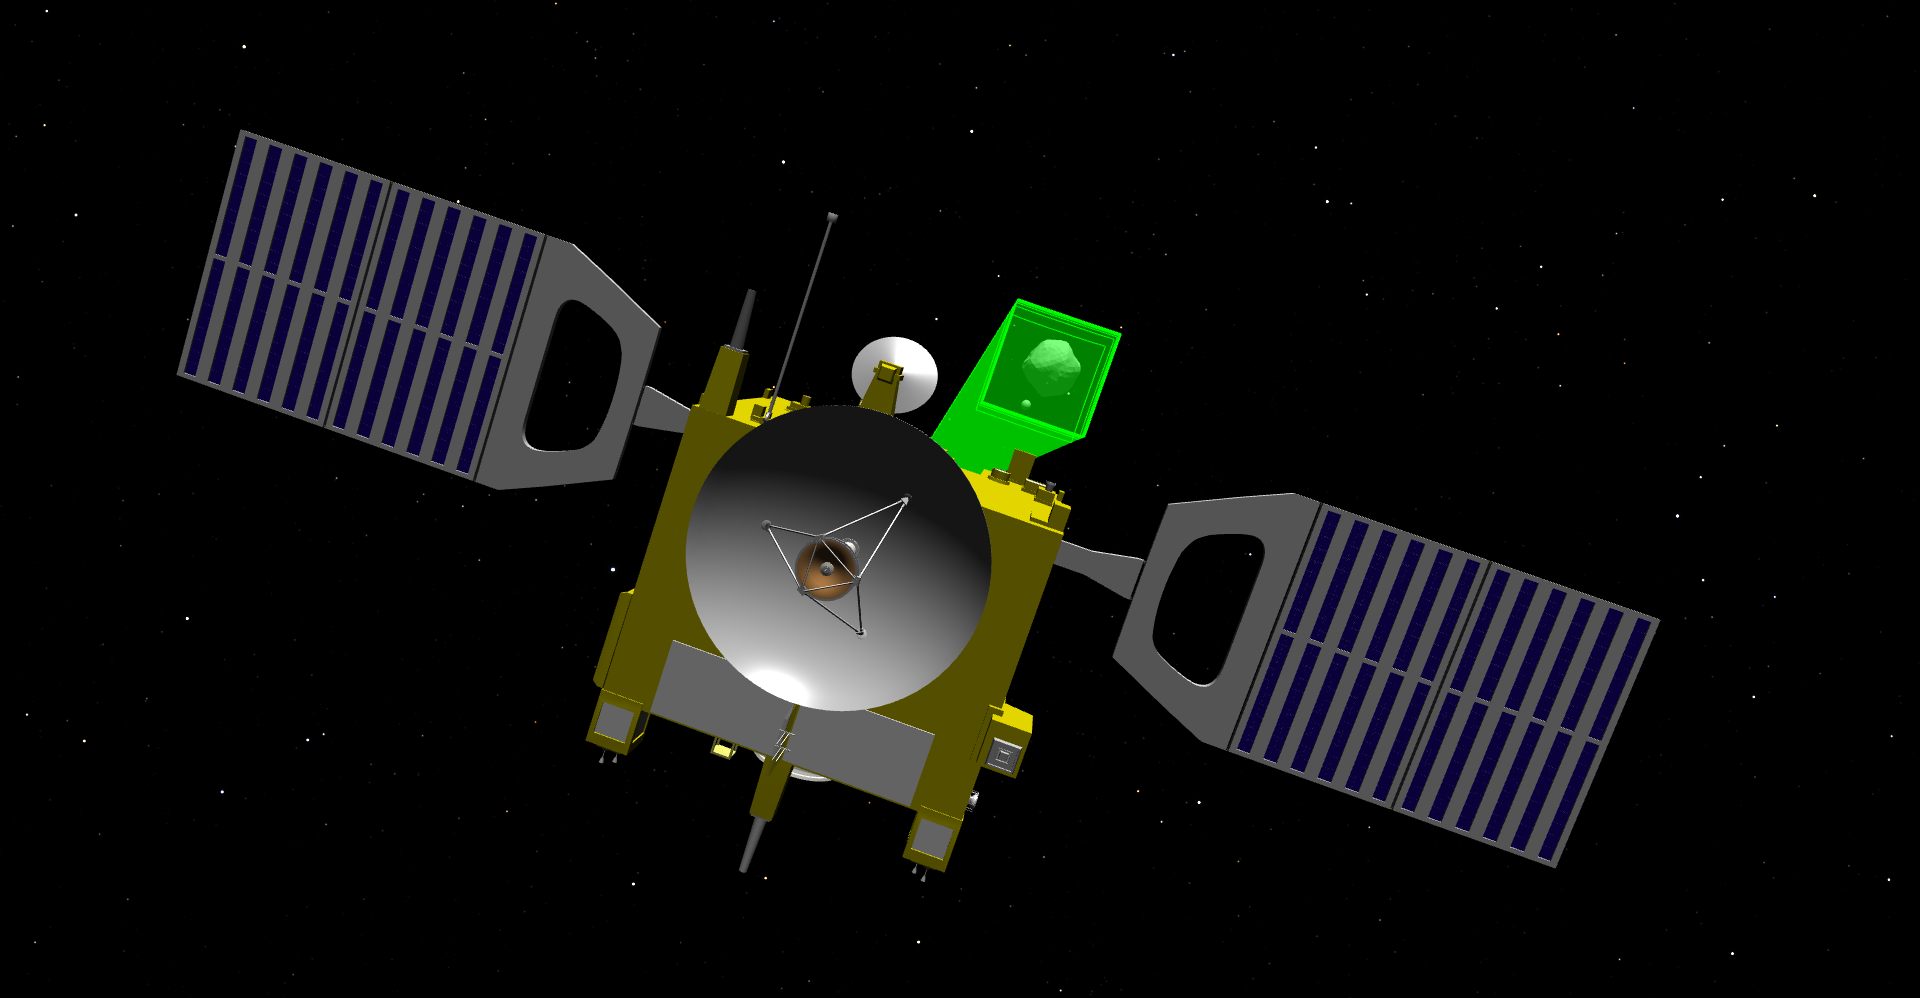
\includegraphics[width=\linewidth]{rsc/hera_didymos.png}
    \caption{The binary system of asteroid Didymos viewed from the spacecraft Hera. The field of view of the AFC camera is in green.}
    \label{fig:1.1}
\end{figure}

\begin{figure*}[b]
    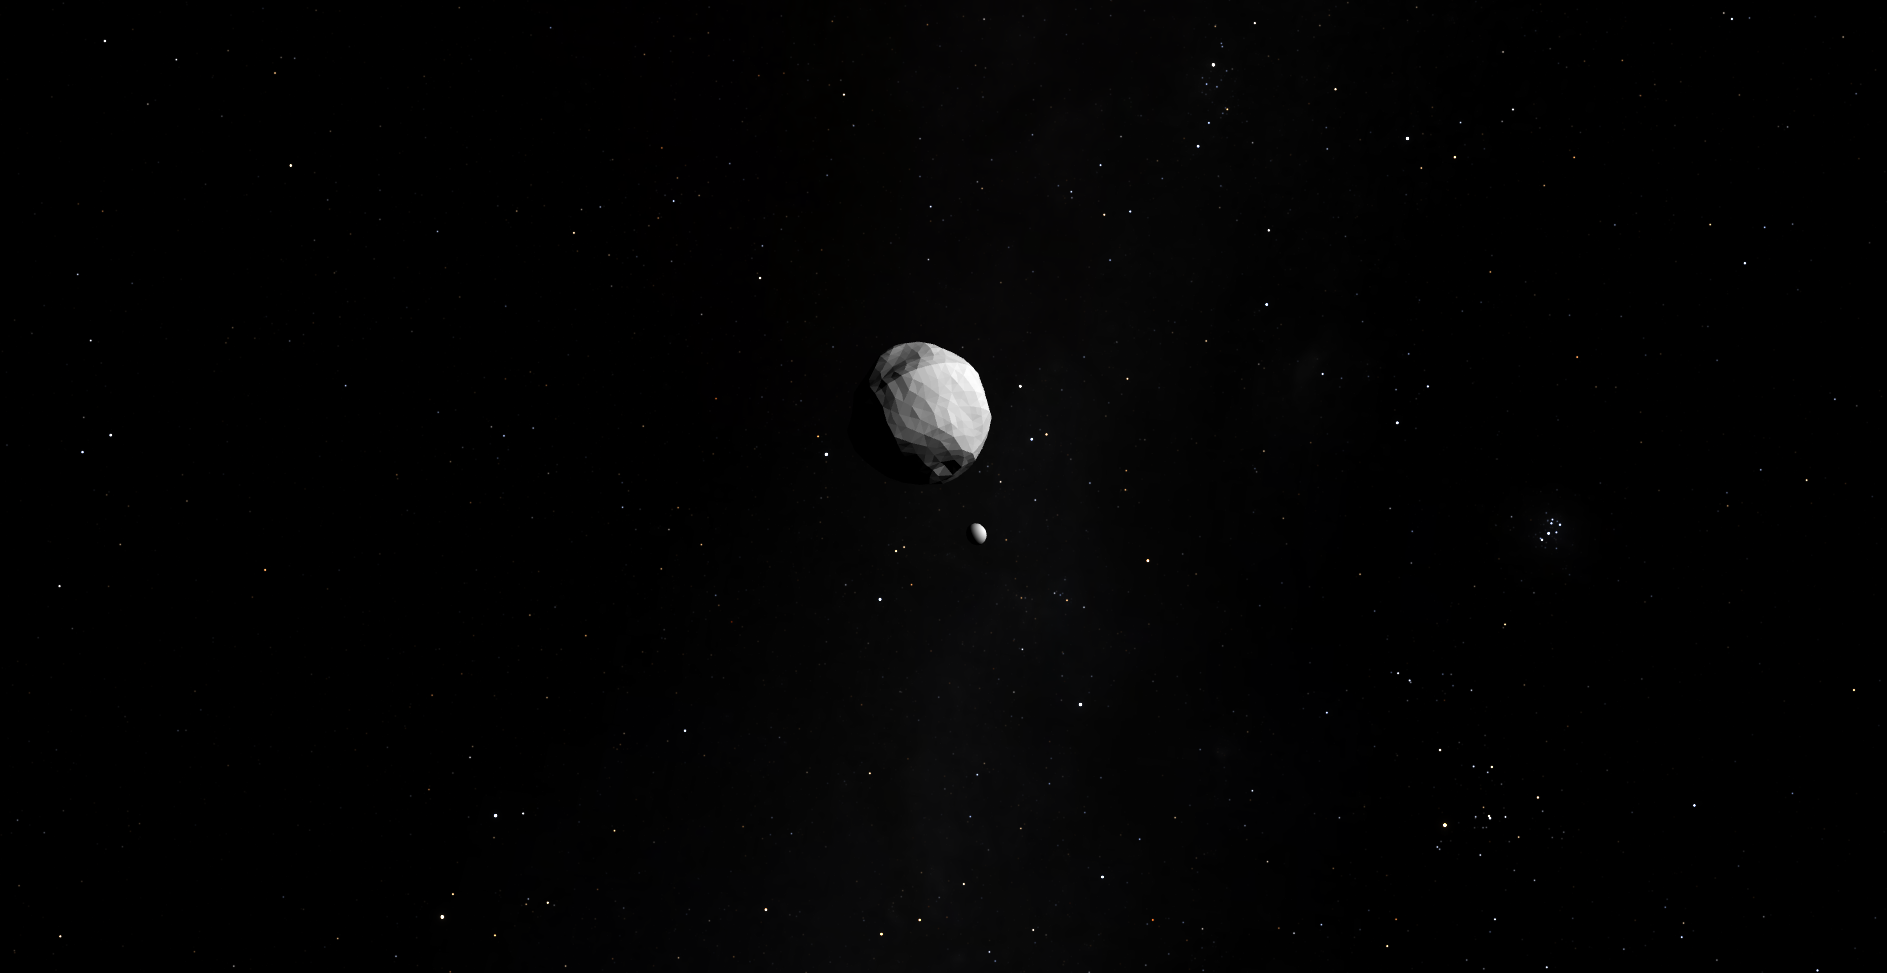
\includegraphics[width=\linewidth]{rsc/didy.png}
    \caption{The binary system of asteroid Didymos}
    \label{fig:1.2}
\end{figure*}
